
\section{Detecção de Áreas de Florestas Pseudo-Invariantes em Séries Temporais Utilizando Algoritmo Random Forest}

\subsection{Introdução}

\hspace{13pt} O monitoramento remoto da paisagem se estabeleceu em nossa sociedade como uma das principais formas de planejamento estratégico e como uma ferramenta importante para a quantificação de recursos e execução de políticas públicas. Os programas de monitoramento de queimadas e de desmatamento ilegal ganham cada vez mais espaço nos noticiários recentes não somente devido a clara relevância dos resultados obtidos, mas também porque seus resultados repercutem diretamente em muitos dos acordos comerciais que os países tem a possibilidade de realizar. 

Dentre todas as possibilidades de uso de ferramentas de sensoriamento remoto para a detecção de mudanças da paisagem, a detecção de mudanças em áreas florestadas focando em eventos de supressão tem um papel importante e possivelmente é uma das mais estudadas e com maior foco na área. Além dos motivos apontados anteriormente, os dados de monitoramento das supressões ocorridas nessas áreas podem ser usados também como dado de entrada para análises que visam a priorização espacial de áreas estratégicas para a conservação e, mais recentemente, para a restauração de áreas com histórico de supressão. Projetos como o Mapbiomas \citep{Souza2019} realizam o mapeamento sistemático do uso do solo para todo o território nacional e a detecção de mudanças de uso ao longo do período do mapeamento (1985 – 2018), sendo um exemplo de como a área de geotecnologias pode se beneficiar com o aumento do acesso à computação de alto desempenho. 

Além disso, devido a esse aumento do poder computacional e de seu acesso, novos algoritmos visando a análise de séries temporais, utilizando imagens digitais orbitais como base, surgiram como uma tentativa de aprimorar, não só a detecção da mudança em si, assim como de sua interpretação, agregando cada vez mais conteúdo de qualidade às análises. Alguns desses algoritmos visam a detecção de mudanças em áreas de floresta como é o caso do CCDC - Continuous Change Detection and Classification \citep{ZHU2014152}, COLD - Continuous Monitoring of Land Disturbance \citep{Cohen2020}, Landtrendr \citep{KENNEDY20102897, KENNEDY2012117}, VCT – Vegetation Change Tracker \citep{Huang2010, THOMAS201119}, EWMACD - Exponentially Weighted Moving Average Change Detection \citep{Brooks2014}, MIICA - Multi-index Integrated Change Analysis \citep{JIN2013159}, VerDET - Vegetation Regeneration and Disturbance Estimates through Time \citep{Hughes2017}, ITRA - Image Trends from Regression Analysis \citep{VOGELMANN201292} e o Shapes-NBR \citep{Meyer2013, Moisen2016}.

Pensando pela perspectiva temporal, é importante entender exatamente qual tipo de mudança se espera obter com a utilização desses algoritmos. Muitas das ferramentas já citadas possibilitam a detecção não somente de eventos de grande magnitude, mas também de processos de degradação que ocorreram ao longo de décadas, ou seja, processos de baixa magnitude, o que possibilita estudos mais elaborados, mas que ao mesmo tempo podem gerar resultados com mais ruído.

Como se pode imaginar, a limpeza dos dados na etapa de pós processamento desses algoritmos acaba sendo essencial para a obtenção de resultados de boa qualidade. É normal que pequenas variações na própria radiometria da imagem sejam detectadas como mudança. Apesar de ser possível retirar grande parte desse ruído considerando apenas mudanças com magnitudes mais altas, áreas de floresta que possuem alta declividade, por exemplo, tendem a sofrer mais com certos ruídos. Sendo assim, parte da limpeza desses dados normalmente acontece utilizando dados gerados por projetos como o Mapbiomas. Os dados do Mapbiomas podem ser utilizados como uma máscara para ignorar áreas de não interesse. Pixels que foram classificados em todos os anos do mapeamento do Mapbiomas como áreas urbanas, corpos d’água, pasto, solo exposto, agricultura e, claro, florestas, são binarizados e multiplicados entre si (classe a classe) para serem utilizados como máscaras com o objetivo de limpar possíveis ruídos no resultado final de um algoritmo como o Landtrendr \cite{KENNEDY2007370, KENNEDY20102897, Kennedy2018}. No entanto, os mapeamentos anuais do Mapbiomas entendem a classificação de forma anual, e não de forma multitemporal, o que pode implicar em erros quando a multiplicação das classificações é realizada para gerar as camadas binárias que servirão para limpar os ruídos. Um pixel que possa ter sido mapeado de forma equivocada em um único ano pode anular a inclusão desta mesma área como uma área a ser utilizada como máscara. Portanto, ao utilizarmos este método, somente áreas bem consolidadas acabam sendo selecionadas para limpar o resultado gerado pelo algoritmo de detecção de mudança.

Sendo assim, o presente trabalho buscou elaborar uma alternativa a esta técnica, apresentando uma forma mais precisa de gerar camadas de áreas de estabilidade, ou seja, áreas que apesar de terem sido afetadas por pequenas mudanças mantiveram alguma característica principal ao longo da série. O foco dado neste trabalho foi para a classe que chamamos aqui de florestas invariantes, já que normalmente é a classe de maior interesse e possivelmente a que possui maior quantidade de ruído associado. Diferentemente do método mais tradicional, a ideia foi realizar a criação de uma máscara gerada a partir da classificação de toda a série temporal e não da agregação de camadas classificadas individualmente ano a ano. 

\subsection{Metodologia}

\hspace{13pt} Para a realização deste trabalho utilizou-se como área de estudo o limite a APA da Bacia Hidrográfica do Rio São João (Figura \ref{fig:bhrsj}). A área foi escolhida por já possuir extenso número de trabalhos de referência publicados e por apresentar elementos da paisagem que representam de forma geral grande parte o contexto morfoclimático e fitogeográfico do Estado do Rio de Janeiro.

\begin{figure}[h!]
    \centering
    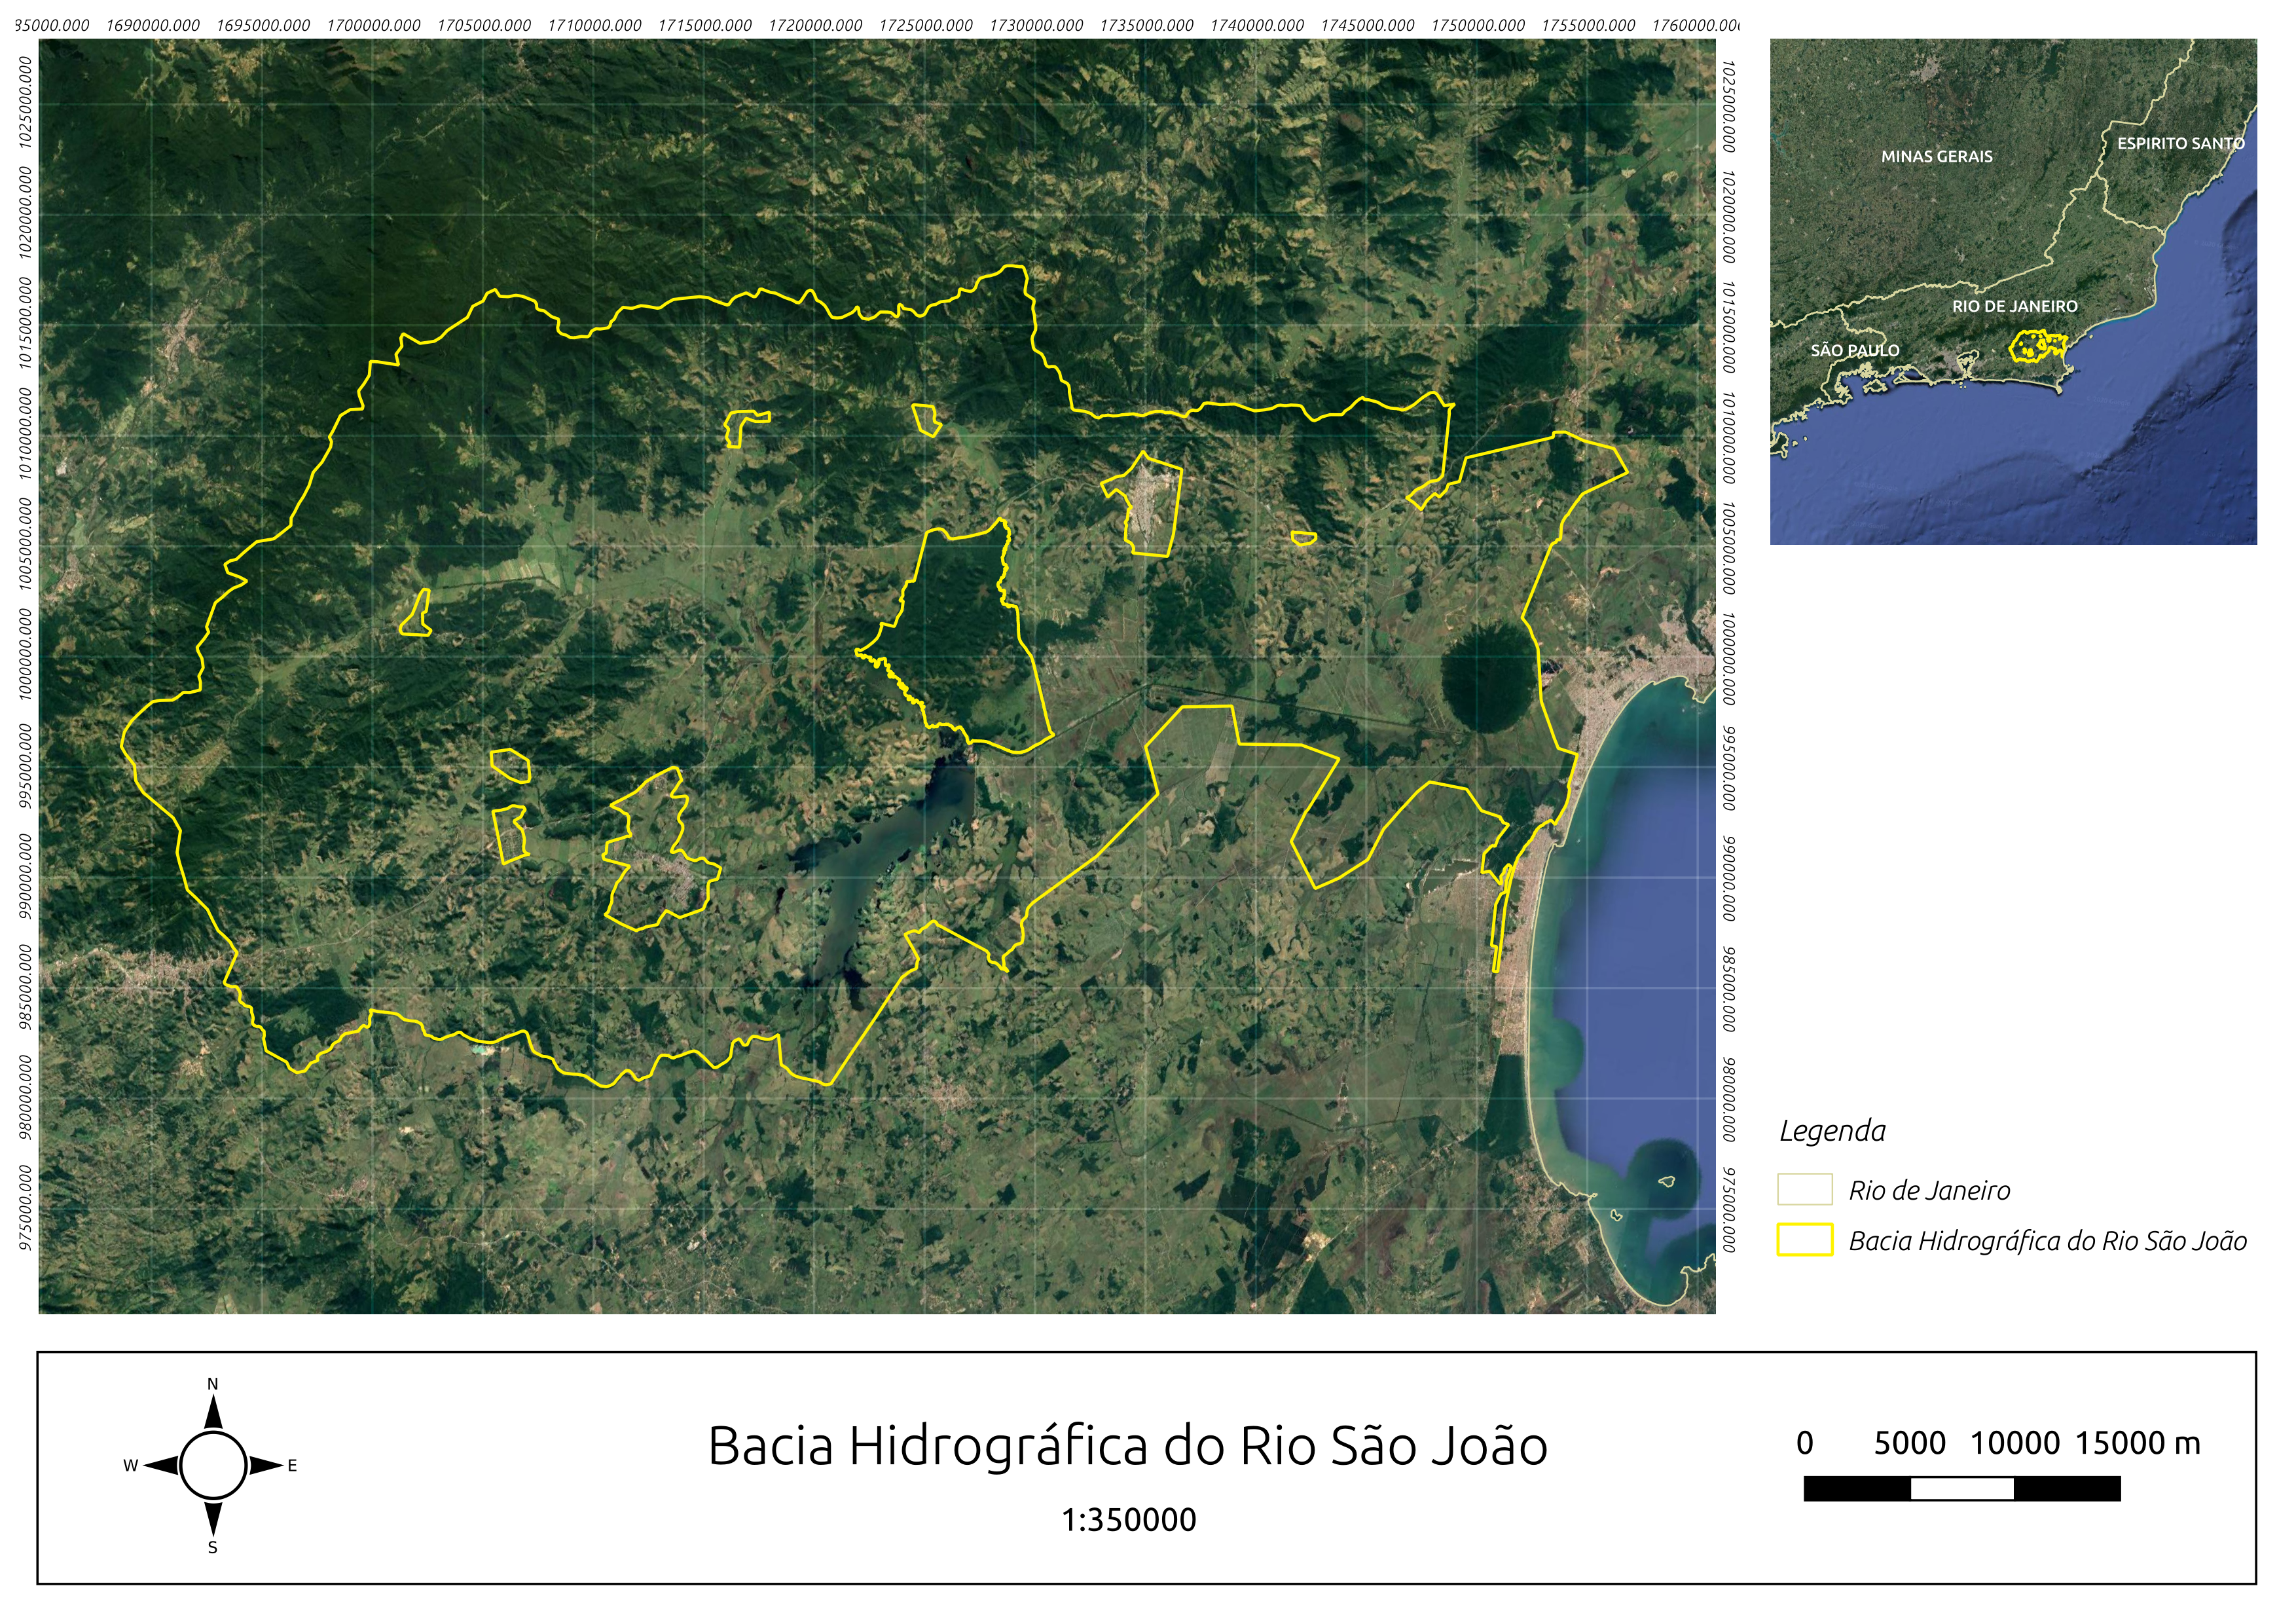
\includegraphics[scale=.5]{images/bhrsj_v2.pdf}
    \caption{O valor de biomassa chegou a ser ainda menor do que quando a maior perda foi registrada.}
    \label{fig:bhrsj}
\end{figure}

Inicialmente foi necessário gerar a camada de floresta invariante utilizando os dados do Mapbiomas. Ou seja, tudo que foi classificado como floresta durante todos os anos do mapeamento. Neste caso, floresta é tudo que foi classificado como “Formação Florestal” pelo Mapbiomas. Para isso, todas as camadas de uso do solo para o bioma da Mata Atlântica gerados pela série 4.1 do projeto (de 1985 até 2018, totalizando 33 camadas) foram recortados de acordo com os limites da APA e passaram por um processo de reclassificação, resultando em camadas binárias (floresta e não-floresta). Após a reclassificação, todas as camadas foram multiplicadas entre si resultando finalmente em uma camada binária final, onde florestas possuem com valor 1 e áreas de não-floresta valor 0.

Como a proposta metodológica consiste na aplicação de um algoritmo de classificação em toda a série temporal, foi essencial a coleta de boas amostras representativas de florestas invariantes. Boas amostras são essenciais para um resultado final satisfatório. Além disso, não seria prudente utilizar somente a camada do Mapbiomas para coletar tais amostras, já que a mesma seria posteriormente comparada com o resultado final. Sendo assim, além da utilização dos próprios dados do Mapbiomas, foi gerada uma imagem sintética do valor máximo de NDVI, considerando todos os anos da série temporal, de forma a realizar uma coleta de amostras através de uma abordagem mais conservadora.

A camada de máximo valor de NDVI foi toda desenvolvida utilizando a plataforma GEE. Para a geração dessa camada foram utilizadas todas as imagens disponíveis do satélite Landsat considerando as séries 5, 7 e 8. Foram utilizadas todas as imagens disponíveis para todos os três satélites presentes na coleção Surface Reflectance Tier 1 por já possuírem correção atmosférica (6S).

Após uma filtragem inicial, aplicou-se uma função em cada uma das imagens (datas) disponíveis, gerando-se uma imagem NDVI correspondente. Através de uma outra função retirou-se todos os pixels com presença de nuvens e sombras.

Com o conjunto total de imagens NDVI, extraiu-se para cada ano da série a mediana dos valores obtidos por pixel e, a partir do novo conjunto gerado, extraiu-se o valor máximo encontrado em toda a série. Desta forma, a camada final representou o valor máximo das medianas de cada ano. A escolha da mediana como um passo intermediário foi crucial para a eliminação de ruídos e valores inválidos presentes na série temporal, dado que o cálculo baseado apenas na extração dos valores máximos gera uma camada final com ruídos espalhados por toda a imagem.

Após a criação da camada de máximo valor de NDVI, buscou-se um limiar para o valor de corte do que poderíamos classificar como floresta. Considerando que os tipos de uso do solo que mais podem gerar confusão em uma classificação com áreas de floresta são as áreas de pastagem e agricultura, uma nova camada contendo somente essas duas classes foi gerada utilizando os mesmos dados do Mapbiomas com a mesma metodologia realizada anteriormente para as áreas de floresta.

Tanto a camada raster de florestas invariantes (Mapbiomas) como a de pasto/agricultura invariantes (Mapbiomas) foram transformadas em pontos (vetor), selecionando-se dois mil destes pontos de forma aleatória para a aplicação de um teste t de Student. A seleção de pontos de forma aleatória se deu desta forma para evitar um possível enviesamento espacial. A aplicação do teste t de Student resultou em um valor-p de 2.2e-16, apresentando, portanto, diferença significativa entre as duas amostras. Com isso é possível concluir que as amostras com os valores de NDVI de florestas tem alta chance de pertencerem a áreas de floresta. Sendo assim, uma função para extrair o valor mínimo presente nas duas mil amostras de florestas foi processada apresentando um valor de 0,83. O valor de 0,83 pode então ser utilizado como valor de limiar de corte (threshold) para a geração de camadas binárias. A multiplicação da camada binária de florestas invariantes do Mapbiomas com a camada binária de máximo NDVI (todos valores maiores que 0.83) serviu então como nossa camada para extração de pontos de floresta para o treinamento do modelo de classificação.

Já para a extração de pontos de florestas que apresentaram alguma mudança significativa, utilizou-se o resultado do algoritmo Landtrendr. A escolha deste algoritmo se deu à sua capacidade de detecção de eventos de baixa magnitude, o que em muitos casos significa a detecção de processos de degradação mais lentos e longos além claro da típica detecção de eventos de grande mudança. Dentre os muitos resultados que o algoritmo oferece, a camada escolhida foi o da detecção dos maiores eventos de perda de vegetação (Greatest Loss) utilizando imagens anuais de 1985 até 2018 e considerando todas as imagens disponíveis para cada ano no período de 1 de janeiro até 31 de dezembro. Como camada padrão utilizou-se o NDVI para o processamento do resultado final.

Após o Landtrendr apresentar o resultado com todas as maiores perdas detectadas, iniciou-se o processo de limpeza desses dados ao considerar apenas as mudanças com magnitudes maiores que 200, ou seja, perdas maiores que 0,2 no NDVI em um único evento. Nenhuma outra limitação foi imposta ao algoritmo e todos os outros parâmetros foram utilizados de forma padrão sem nenhuma modificação.

Já os pontos para a classe “outros” (água, solo exposto, pasto, etc.) foram coletados de forma aleatória utilizando a imagem resultante com todos os pixels que não tinham sido classificados anteriormente nem como floresta pela fusão da camada do Mapbiomas com o NDVI máximo, e nem pelos pixels detectados pelo Landtrendr como áreas com possível perda de vegetação.

Todas as amostras das três classes foram então importadas em formato shapefile para a plataforma do Google Earth Engine (GEE) para execução do processo de classificação utilizando o algoritmo Random Forest. Como imagem base para a classificação foi necessário ter uma série temporal com imagens anuais seguindo os mesmos padrões da série do Mapbiomas para possibilitar posterior comparação. Essa série de imagens foi gerada utilizando um script desenvolvido no GEE contendo, para cada ano, uma composição de valores considerando o valor da mediana de cada pixel para cada banda. Para cada ano foram utilizadas as bandas Blue, Green, Red, NIR, SWIR1, SWIR2 e também de índices como o NDVI, NDWI, NDMI, SAVI, Greenness, Wetness e Brightness. Áreas com nuvens e sombra foram mascaradas com valores “no data” e, portanto, não foram consideradas no cálculo da mediana.

No entanto, por se tratar de uma nova metodologia, antes de gerar o processo de classificação final utilizando as amostras coletadas, escolhemos realizar testes de validação cruzada (cross validation) para entender melhor quais variáveis (bandas) teriam o melhor desempenho ao classificar este tipo de classe. Utilizamos então as amostras coletadas (250 pontos/classe) para extrair os valores da série temporal e exportamos para um ambiente offline, já que atualmente não existem ferramentas de teste e validação suficientemente boas no GEE.

As tabelas com os valores das amostras foram processadas no pacote MLR (Machine Learning in R) (BISCHL, et al., 2016) utilizando o classificador Random Forest com 100 árvores cada e com a validação cruzada em modo “k-fold” utilizando parâmetro 10 (divide o subconjunto das amostras em 90\% treino e 10\% teste), repetindo ainda o processo por 100 iterações para cada teste, obtendo então um único valor de índice kappa por teste. Cada rodada aqui representa uma combinação de bandas a serem utilizadas pelo classificador para tentar separar as três classes. Para este teste foram consideradas 24 combinações diferentes de bandas. Aplicando o Random Forest para as 24 variações de entrada com o processo de validação cruzada utilizando 10 “folds” e 100 iterações para cada validação, foram gerados 24000 processos de classificação diferentes, com cada processo gerando 100 árvores de decisão (Figura \ref{fig:fluxograma}). Os resultados para essa quantidade exaustiva de testes são os apresentados na Tabela \ref{tab:1}:


\begin{table}[h!]
\centering
\rowcolors{2}{red!50!yellow!30}{green!40!yellow!10}
\footnotesize
\begin{tabular}{|c | c|}
\hline
                                                               BANDA &  Kappa \\
\hline
    Blue + Green + Red + NIR + SW1 + SW2 + NDVI + NDWI + NDMI + SAVI &  0.844754 \\
Blue + Green + Red + NIR + SW1 + SW2 + NDVI, NDWI + NDMI + SAVI + TC &  0.839872 \\
                                Blue + Green + Red + NIR + SW1 + SW2 &  0.838804 \\
                                            Blue + Green + Red + NIR &  0.833381 \\
                                                  Blue + Green + Red &  0.832774 \\
         Greeness + Wetness + Brightness + NDVI + NDWI + NDMI + SAVI &  0.829503 \\
                                                   NDVI + NIR + NDMI &  0.819875 \\
                                                          NDVI + NIR &  0.819833 \\
                                     Greeness + Wetness + Brightness &  0.812621 \\
                                                                 Red &  0.812496 \\
                                                               SWIR2 &  0.808915 \\
                                                              Green  &  0.805528 \\
                                                                Blue &  0.800079 \\
                                           NDVI + NDWI + NDMI + SAVI &  0.796679 \\
                                                         NDVI + NDMI &  0.783342 \\
                                                               SWIR1 &  0.778846 \\
                                                             Wetness &  0.767554 \\
                                                           Greenness &  0.761319 \\
                                                               NDVI  &  0.755475 \\
                                                                SAVI &  0.755282 \\
                                                          Brightness &  0.715955 \\
                                                                NDMI &  0.706022 \\
                                                                NDWI &  0.634395 \\
                                                                 NIR &  0.576071 \\
\hline
\end{tabular}
\caption{Índice Kappa para as Combinações de Variáveis Utilizadas. (SW1 = SWIR1, SW2 = SWIR2, TC = Tasseled Cap = Greeness, Wetness, Brightness)}
\label{tab:1}
\end{table}

\newpage

\begin{figure}[h!]
    \centering
    \includegraphics[scale=.4]{images/fluxograma.pdf}
    \caption{Fluxograma demonstrando o processo de validação cruzada. Todo o processo foi repetido para cada combinação de banda utilizada no estudo, totalizando 24 processos independentes.}
    \label{fig:fluxograma}
\end{figure}

É importante frisar que o processo de validação cruzada representa apenas uma etapa intermediária antes da classificação final que visa uma melhor escolha dos parâmetros ao verificar através de muitos testes qual combinação de variáveis obteve melhor resultado (menor erro).

Observa-se que a melhor combinação de bandas para o processo de classificação não é a simples utilização de todas as bandas. A incorporação do Tasseled Cap não trouxe uma melhoria na precisão do modelo. No entanto, a tabela de desempenho também apresenta outros resultados interessantes, como por exemplo a taxa de acerto utilizando apenas a banda do vermelho (Red) ou em como bandas que são tipicamente usadas pela comunidade de forma ampla para detecção de áreas vegetadas como o NDVI, NDMI e SAVI apresentaram resultados piores do que muitas outras combinações possíveis. 

\subsection{Resultados}

\hspace{13pt} Após a otimização do modelo, foi feita uma seleção na série temporal para utilizar apenas a combinação de bandas que obtiveram o melhor resultado (Blue, Green, Red, NIR, SWIR1, SWIR2, NDVI, NDMI, NDWI e SAVI) e assim gerar uma classificação final (Figura \ref{fig:bhrsj_class_final}). Como resultado obtivemos uma área total de florestas invariantes na APA, de 501,1km2.

\begin{figure}[h!]
    \centering
    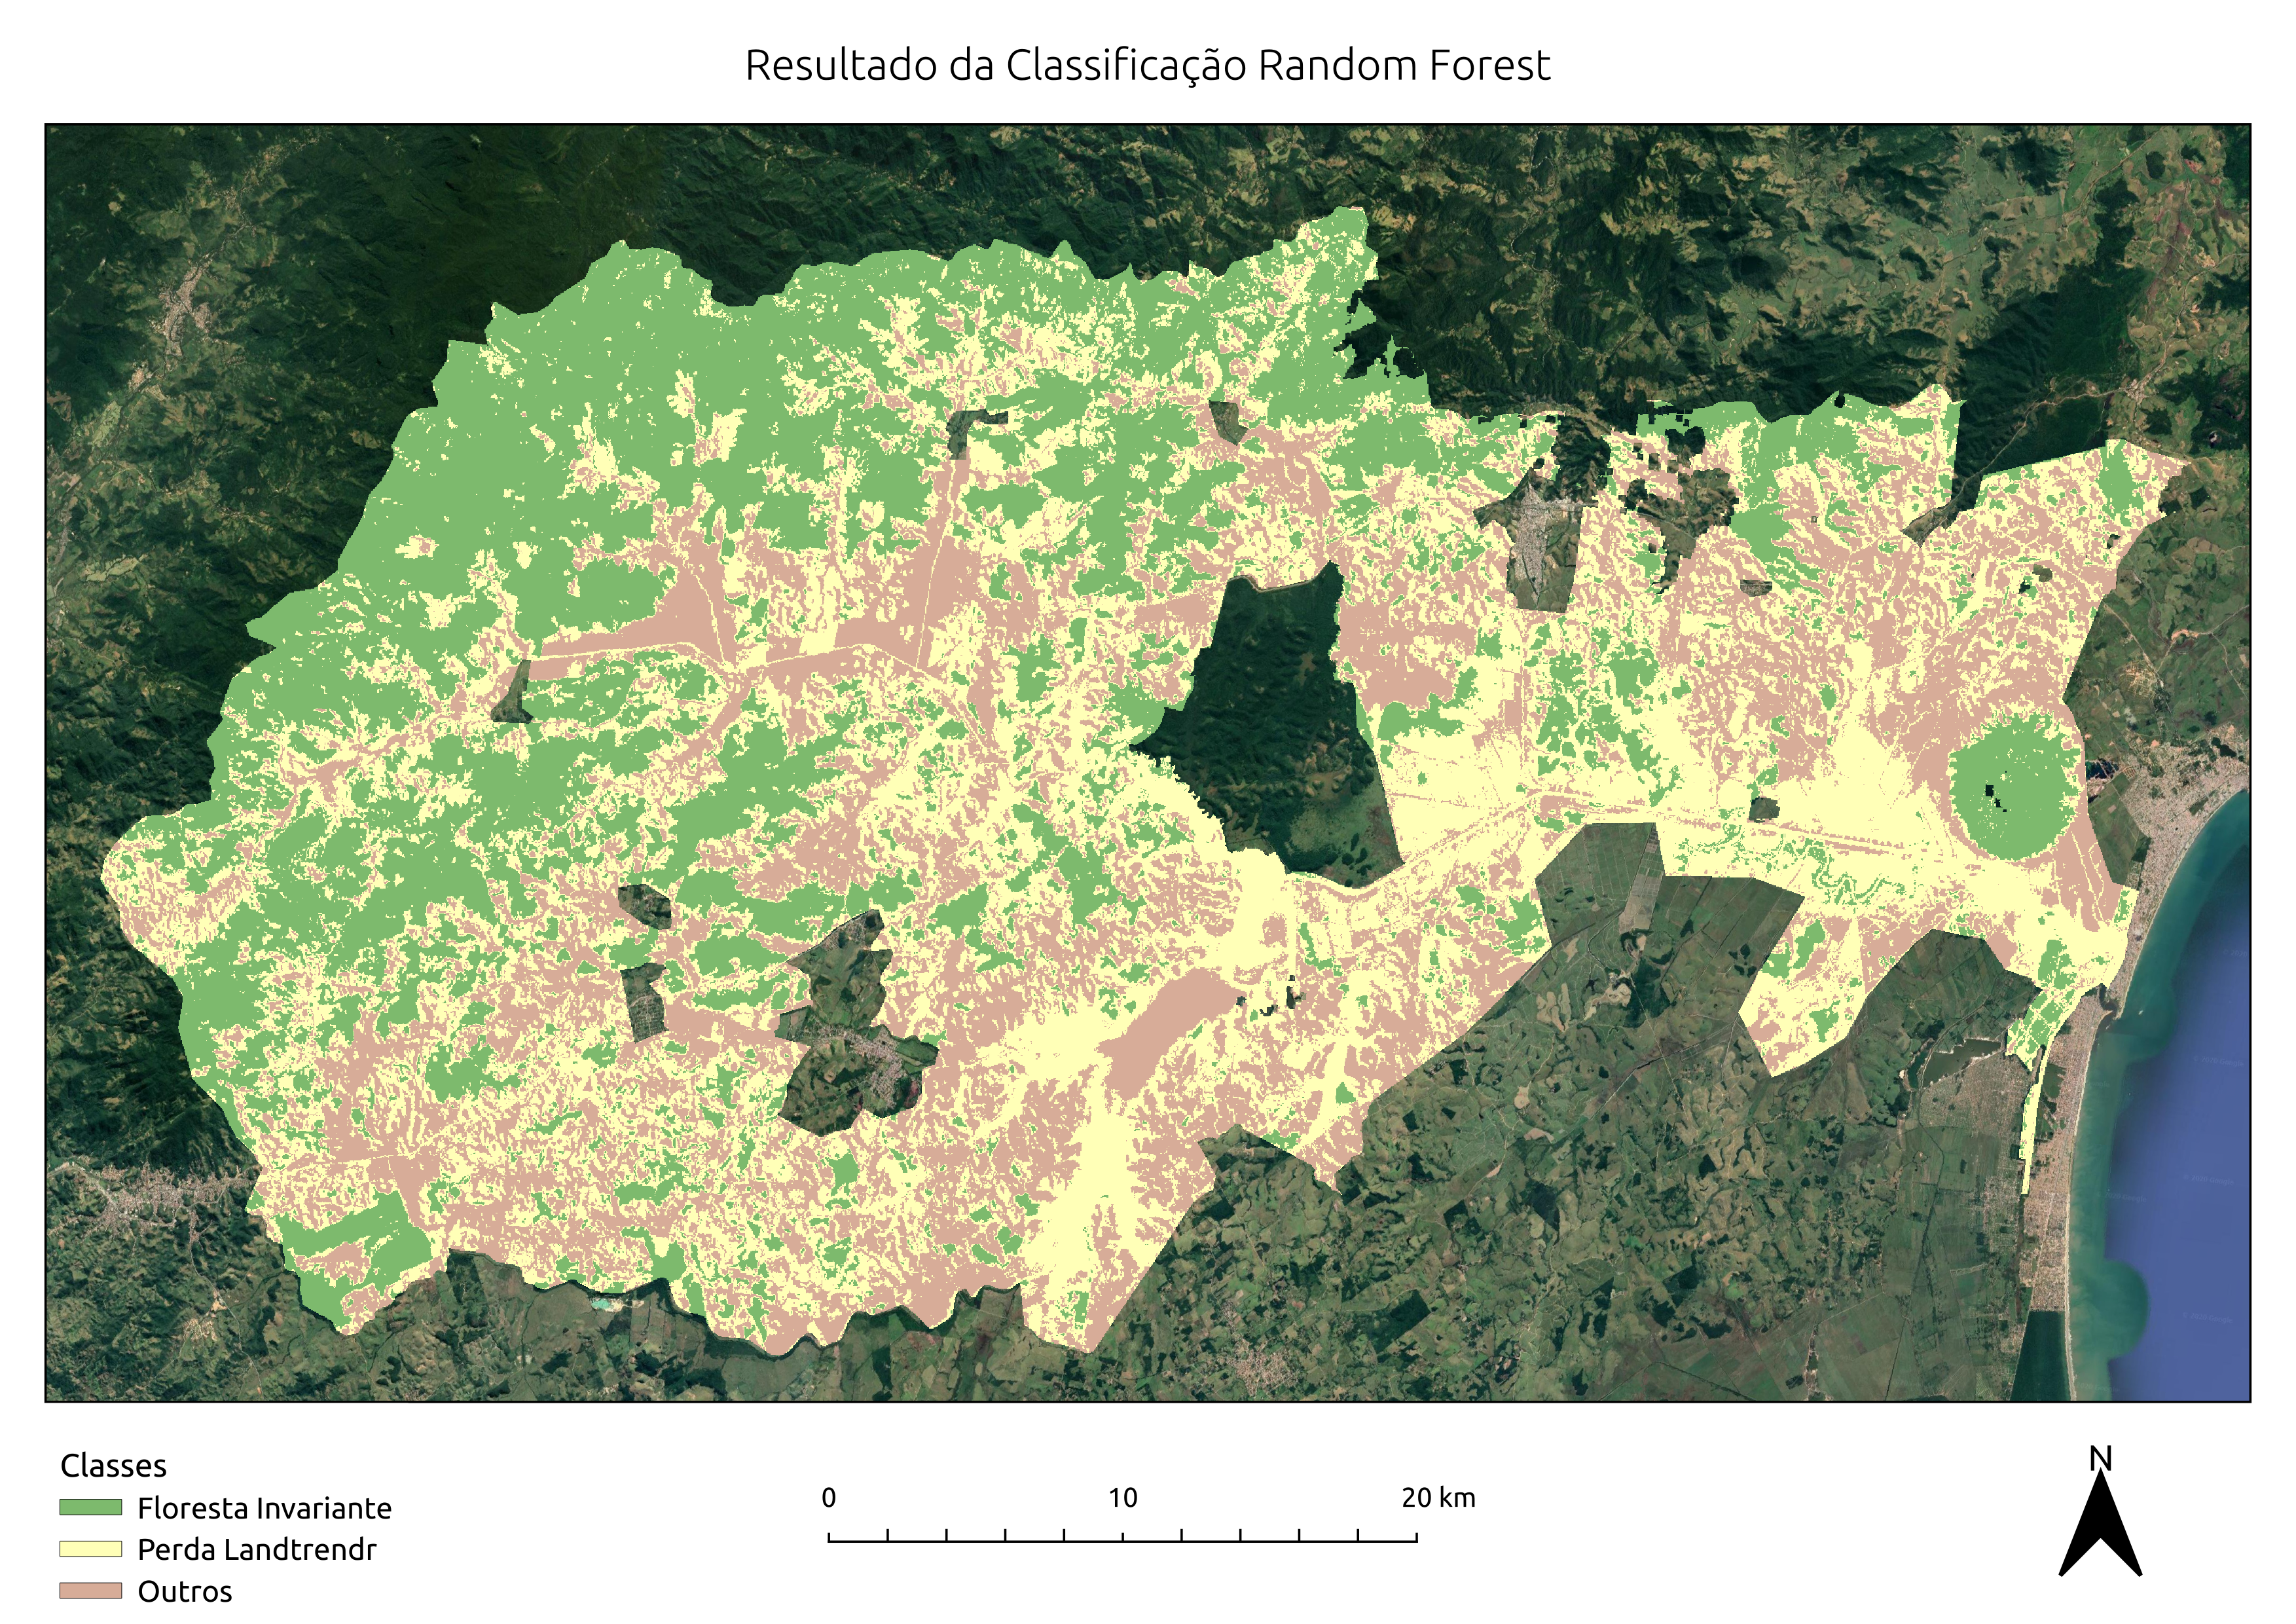
\includegraphics[scale=.5]{images/bhrsj_class_final.pdf}
    \caption{Classificação final gerada no Google Earth Engine (Classificação final)}
    \label{fig:bhrsj_class_final}
\end{figure}

\newpage

As classes escolhidas para o mapeamento final foram “Floresta Invariante”, “Perda Landtrendr” e “Outros”. A classe “Floresta Invariante” representa todos os pixels que mantiveram algum grau de coerência espectral ao longo da série temporal. Mesmo com algumas variações ao longo do tempo, o classificador pode encontrar padrões e descartar anomalias da série. Este comportamento é importante justamente para descartar ruídos presentes em qualquer série temporal sem a necessidade da aplicação de outros algoritmos de pré-processamento e por já garantir um bom resultado. Já a classe “Perdas Landtrendr” foi fortemente influenciada pelo resultado do algoritmo Landtrendr que já tinha detectado os padrões de perda (loss) anteriormente. Ou seja, é importante garantir que o resultado do algoritmo de detecção de mudanças seja o melhor possível modificando seus parâmetros de acordo com a área de estudo. Por fim, a classe “Outros” representa todas as outras classes presentes na bacia e que foram agregadas para não gerar confusão com os objetivos do mapeamento. O resultado da classificação final foi bastante satisfatório, apresentando um padrão espacial das classes esperado para a área de estudo.

No entanto, além da classificação gerada, uma nova imagem teve de ser criada para a comparação entre o resultado obtido pelo Random Forest e a imagem binária utilizando somente dados do Mapbiomas. A nova imagem foi criada somando-se a camada de florestas invariantes com todos os anos do Mapbiomas com a versão binarizada do resultado final (florestas invariantes - outros).

Com essa imagem fusionada pode se notar que grande parte dos pixels (469,8km2 ou 76,9\% da área mapeada) foram classificados como floresta invariante tanto pelo Random Forest como pelo Mapbiomas. No entanto, diferenças como áreas onde somente o Random Forest classificou como floresta (22,7km2 ou 3,8\% da área mapeada) e onde somente o Mapbiomas classificou como floresta (52,7km2 ou 8,7\% da área mapeada) também foram detectadas. Os outros 10,8\% de área restantes foram excluídos da análise por não serem áreas de interesse.

Para entender melhor a qualidade de cada resultado, foram feitos alguns testes estatísticos. Primeiramente, foram selecionadas duas mil amostras aleatórias de três classes: Áreas que foram classificadas como floresta pelos dois mapeamentos (FOR), áreas que foram classificadas como floresta apenas pelo Random Forest (RF) e áreas que foram classificadas como floresta apenas pelo Mapbiomas (MB). Um teste de análise de variância (ANOVA) foi realizado para entender se os valores encontrados por cada amostra eram estatisticamente similares. O valor-p obtido pela ANOVA foi de 0,0116, o que mostrava uma diferença significativa entre as amostras considerando um limiar de valor-p de 0,05. Sendo assim, buscou-se então realizar um teste entre cada uma das amostras utilizando o teste de Tukey \citep{Tukey1949}. Os resultados são os apresentados na Tabela 2.

\begin{table}[h!]
    \centering
    \begin{tabular}{|c | c|}
    Combinação (Teste de Tukey) &  Valor-p      \\
                Mapbiomas - FOR &  8.489000e-04 \\
                       RF - FOR &  1.841643e-01 \\
                 RF - Mapbiomas &  2.000000e-07 \\
    \end{tabular}
    \caption{Resultados do Teste de Tukey}
    \label{tab:2}
\end{table}

Os resultados foram considerados promissores. Segundo o teste de Tukey, ao mesmo tempo em que as amostras que somente o Mapbiomas mapeou como floresta invariante são significativamente diferentes das que ambos os mapeamentos mapearam como floresta invariante. Já as amostras do Random Forest que são diferente das do Mapbiomas, quando comparadas com as mapeadas por ambos, são estatisticamente similares.

Este resultado mostra que a classificação feita pela metodologia proposta apresenta um resultado possivelmente superior a obtida utilizando somente as camadas do Mapbiomas. No entanto, ainda seria preciso saber o quanto de erro associado poderia existir, não apenas nas áreas mapeadas pelo Mapbiomas ou pelo Random Forest, mas também nas áreas em que ambos obtiveram o mesmo resultado.

Para este processo de validação final utilizamos a ferramenta TimeSync \citep{COHEN20102911}. Diferente do processo de validação comum nos mapeamentos de apenas uma ou poucas datas, a validação de séries temporais densas necessita de ferramentas especiais como o TimeSync, que apesar de ter utilização ainda consideravelmente complexa, é uma das únicas ferramentas existentes que realizam esse tipo de validação. 

O TimeSync funciona de forma integrada com o GEE e também necessita do software Access da Microsoft para armazenar as coordenadas de cada ponto a ser validado. A validação do TimeSync é feita de forma visual através da interface gráfica do programa.

Foram coletados para a etapa de validação no TimeSync trezentos pontos para cada uma das classes. Os pixels mapeados apenas pelo Mapbiomas tiveram uma taxa de acerto de 55\%, enquanto os pixels mapeados pelo Random Forest tiveram uma taxa de acerto de 76\%. Já os pixels mapeados por ambos tiveram um acerto de 97\%. Logo após, um último teste foi realizado considerando outras trezentas amostras do mapa final gerado pela nova metodologia, mas considerando apenas os pixels que foram classificados como floresta invariante, resultado em uma taxa de acerto final de 91,7\%. Todos os resultados, amostras, imagens, arquivos vetoriais, códigos e materiais para validação utilizados neste trabalho estão disponíveis para visualização e possível replicação através deste link: \url{https://github.com/sacridini/florestas\_invariantes\_random\_forest}.

\subsection{Conclusões}

\hspace{13pt} Através dos testes realizados neste trabalho podemos verificar que a metodologia proposta apresentou melhor desempenho se comparada à utilização da base de dados do Mapbiomas, quando o objetivo é gerar camadas de florestas que não sofreram nenhuma ou pouca variação ao longo de tempo. É importante lembrar que o Mapbiomas continua sendo uma excelente referência para estudos envolvendo séries temporais, e que a comparação feita visa obter resultados melhores para uma classe que não é oficialmente mapeada pelo projeto já que o mesmo possui objetivos distintos. Os resultados obtidos poderão ser utilizados como base para outros mapeamentos de áreas florestadas invariantes em ambientes tropicais. O trabalho buscou também contribuir para um melhor entendimento das variáveis que melhor conseguem separar classes tão novas como a proposta, já que ainda são poucos os trabalhos que buscam classificar séries temporais nessa escala. Além disso, resultados surpreendentes como o desempenho da banda do vermelho mostram que a utilização de apenas uma única banda pode ser o suficiente para a identificação de áreas similares e servem como um estímulo a novos estudos que visem a detecção de áreas invariantes de forma rápida e pouco custosa.

Máscaras de áreas invariantes como a gerada pelo algoritmo de aprendizado de máquina poderão servir, não só como parâmetros para estudos aplicados à conservação, mas também como máscaras para a limpeza de dados indesejados em resultados obtidos por algoritmos de detecção de mudanças como o Landtrendr e outros.